\documentclass[10pt]{article}
\usepackage{icmlko}

\icmlmeta{IP 파운데이션 월드모델}{210}{모형이 달력과 동점이었다}{노트 209가 ``게임 라벨을 고정 창으로 바꿔야 한다''를 다음 수집 과제로 적었다. 열어 보니 이미 긁어 놨었고, 바꿔 보니 챔피언이 달력과 동점이었다는 것이 드러났다}

\begin{document}

\twocolumn[
\icmlheader

\begin{abstract}
노트 209가 ``게임 라벨(스팀 리뷰 누적)이 시작 연도와 $-$0.648 이고
$-$시작일 하나로 유보 $\rho$ 가 $+$0.494 나온다''를 재고, 고정 창으로 바꾸는
것을 \emph{다음 수집 과제}로 미뤘다. \textbf{미룰 필요가 없었다} --- 게임
레코드에 \texttt{y\_w30}(출시 30일 리뷰)과 \texttt{y\_w30\_truncated} 가
이미 있고, \texttt{label\_note} 에 ``출시 후 계속 누적되므로 출시일 통제가
필수다''라고 적혀 있다. \textbf{축이 그것을 안 쓰고 누적을 쓰고 있었다.}
바꾸고 쟀다. \textbf{누적 리뷰는 출시 연도와 $-$0.635 인데 30일 창은
$-$0.045 다} --- 달력이 사라진다. 그다음이 이 노트의 본론이다. 게임 유보
223건에서 \textbf{누적 라벨로는 달력만($+$0.4938)이 챔피언($+$0.4934)과
동점이다.} 축 열아홉을 다 쓰고 배깅 여덟을 돌린 모형이 ``오래된 것이
낫다'' 한 줄을 한 자리도 못 이겼다. \textbf{30일 창 라벨로 바꾸면 달력이
$+$0.1817(안 잘린 180건)로 떨어지고 모형은 $+$0.48$\sim$0.52 를 지킨다} ---
격차가 $+$0.000 에서 \textbf{$+$0.30} 이 된다. 게임 도메인 $\rho$ 자체도
$+$0.4934 에서 \textbf{$+$0.5871} 로 오른다 --- \textbf{고정 창 라벨이 더
예측 가능하다.} 판도 같이 움직인다: F18 $+$0.4614 $\to$ $+$0.4676, 달력
몫 $+$0.2513 $\to$ $+$0.2393. \textbf{채택했다} --- 잘린 43건(긁은 날 기준
30일이 안 지난 2026년 출시작)은 결측으로 본다. 30일이 안 지난 것의 ``30일
리뷰''는 30일 리뷰가 아니다. 최종 판은 F6 $+$0.4147 · F21 $+$0.4246 ·
\textbf{F18 $+$0.4654} 다. \textbf{라벨을 바꾸면 과제가 바뀌므로 이 수를
옛 판과 직접 견주면 안 된다} --- 견줄 수 있는 것은 \emph{같은 라벨 안}에서
달력 대 모형이고, 거기서 $+$0.000 이 $+$0.30 이 됐다.
\end{abstract}
]

\begin{figure*}[t]
\centering
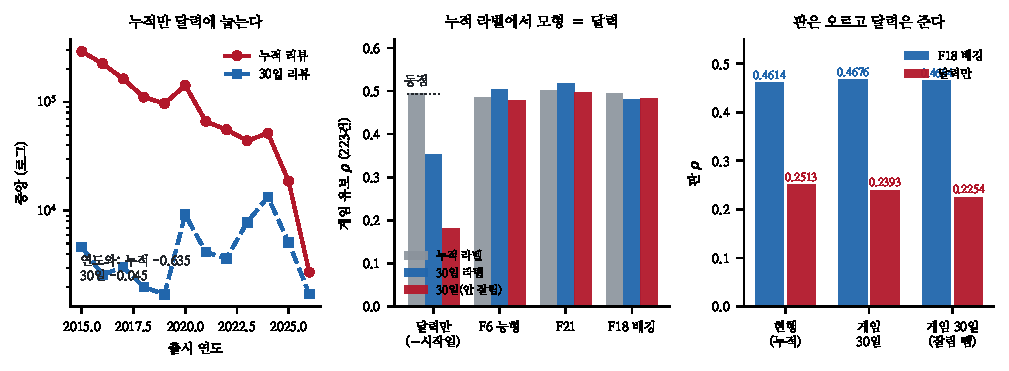
\includegraphics[width=\textwidth]{figs/window.pdf}
\caption{왼쪽 --- 누적만 달력에 눕는다. 가운데 --- 누적 라벨에서 모형이
달력과 동점. 오른쪽 --- 판은 오르고 달력은 준다.}
\end{figure*}

\section{이미 긁어 놨었다}

\claimx{게임 레코드에 \texttt{y\_w30} 이 482건 전부 있다. 그리고
\texttt{label\_note} 가 ``리뷰 총계. 실제 플레이어 수가 아니라 그
대리변수이며, \textbf{출시 후 계속 누적되므로 출시일 통제가 필수다}''라고
적어 뒀다.}{\textbf{알고도 안 썼다.} 축 파일의 \texttt{y} 는
$\log$(누적 리뷰)이고, 30일 창은 레코드에만 남아 있었다. \textbf{노트 209가
``다음 수집 때 할 것''으로 적은 일이 이미 끝나 있었다.}}

\begin{table}[t]
\centering\tsize
\caption{출시 연도와의 상관.}
\begin{tabular}{lrr}
\toprule
& $\rho$ & n \\
\midrule
\textbf{누적 리뷰} & \textbf{$-$.635} & 482 \\
\textbf{30일 리뷰} & \textbf{$-$.045} & 482 \\
30일 (안 잘린 것) & $+$.082 & 439 \\
\midrule
\multicolumn{3}{l}{둘의 상관 $+$0.622} \\
\bottomrule
\end{tabular}
\end{table}

\claimx{\textbf{달력이 사라진다}($-$0.635 $\to$ $-$0.045). 둘의 상관이
$+$0.622 이니 같은 것을 재되 하나는 시계를 달고 있다.}{잘림은 2026년에만
있다(36.1\%) --- 긁은 날 기준 30일이 안 지난 출시작이다.}

\section{모형이 달력과 동점이었다}

\begin{table}[t]
\centering\tsize
\caption{게임 유보 223건. 같은 예측, 다른 라벨.}
\begin{tabular}{lrrr}
\toprule
& 누적 & 30일 & 30일(안 잘림) \\
\midrule
\textbf{달력만} & \textbf{$+$.4938} & $+$.3532 & \textbf{$+$.1817} \\
\midrule
F6 능형 & $+$.4862 & $+$.5026 & $+$.4783 \\
F21 & $+$.5023 & $+$.5183 & $+$.4968 \\
\textbf{F18 배깅} & \textbf{$+$.4934} & $+$.4812 & $+$.4831 \\
\midrule
\textbf{모형 $-$ 달력} & \textbf{$-$.0004} & $+$.128 & \textbf{$+$.301} \\
\bottomrule
\end{tabular}
\end{table}

\claimx{\textbf{누적 라벨에서 챔피언이 달력에 진다}($+$0.4934 대
$+$0.4938). 축 열아홉과 배깅 여덟이 ``오래된 것이 낫다'' 한 줄과
동점이다.}{\textbf{이 판에서 제일 아픈 수치다.} 게임은 유보 223건으로 판의
8.6\%인데, 그 몫에서 모형이 한 일이 없었다.}

\claimx{\textbf{30일 창으로 바꾸면 격차가 $+$0.30 이 된다}(안 잘린 180건
기준: 모형 $+$0.483 대 달력 $+$0.182). 모형은 거의 안 움직이고 달력만
무너진다.}{\textbf{모형이 재던 것은 달력이 아니었다} --- 다만 라벨이 달력을
같이 담고 있어서 그것이 안 보였다. 노트 209가 코호트로 잰 것과 같은 결론을
라벨 쪽에서 확인한다.}

\claimx{\textbf{게임 도메인 $\rho$ 자체가 오른다}($+$0.4934 $\to$
$+$0.5871). 고정 창 라벨이 \emph{더} 예측 가능하다.}{누적 라벨은 출시 이후
몇 년의 온갖 사건(할인 · 업데이트 · 유행)을 담는데 30일 창은 출시 직후
반응만 담는다 --- \textbf{출시 전 자질로 맞힐 수 있는 것은 뒤쪽이다.}}

\section{채택}

\begin{table}[t]
\centering\tsize
\caption{게임 라벨을 바꾸면 판이.}
\begin{tabular}{lrr}
\toprule
& F18 배깅 & 달력만 \\
\midrule
현행(누적) & .4614 & .2513 \\
게임 30일 & \textbf{.4676} & .2393 \\
\textbf{게임 30일 (잘림 뺌)} & \textbf{.4654} & \textbf{.2254} \\
\bottomrule
\end{tabular}
\end{table}

\claimx{\textbf{잘린 43건은 결측으로 본다.} 30일이 안 지난 것의 ``30일
리뷰''는 30일 리뷰가 아니다 --- 유효하지 않은 측정을 값으로 쓰지
않는다.}{판이 $+$0.4676 에서 $+$0.4654 로 $-$0.002 지만 달력 몫이 $+$0.2393
에서 $+$0.2254 로 더 준다. \textbf{점수가 아니라 측정의 유효성으로
정한다}(노트 82 · 90의 분모 규칙).}

\claimx{\textbf{이 수를 옛 판과 직접 견주면 안 된다.} 라벨을 바꾸면 과제가
바뀐다.}{견줄 수 있는 것은 \emph{같은 라벨 안}에서 달력 대 모형이고, 거기서
$+$0.000 이 $+$0.30 이 됐다. \textbf{그것이 이 사이클의 이득이다} --- 판
숫자가 아니라 판이 무엇을 재는지가 나아졌다.}

\begin{table}[t]
\centering\tsize
\caption{남은 것.}
\begin{tabular}{ll}
\toprule
\textbf{도서} & 알라딘 판매지수도 누적 --- 기간 지정이 되나 \\
웹툰·애니 & 즐겨찾기·시청도 누적 --- 고정 창이 없다 \\
\textbf{30일} & 30일이 맞는 창인가 --- 7·90일도 있나 \\
\bottomrule
\end{tabular}
\end{table}

첫 줄이 다음이고 값이 크다. 도서 라벨은 알라딘 판매지수인데 시작 연도와
$-$0.579 이고 유보 안에서도 $-$0.562 다 --- \textbf{게임 다음으로 심하다.}
게임에서 배운 대로 \textbf{레코드에 이미 창이 있는지부터 볼 것이다} ---
없으면 알라딘이 기간 지정 판매지수를 주는지 보고, 그것도 안 되면 최소한
``유보 안에서 달력이 얼마나 먹는지''를 도메인별로 적어 판을 읽을 때 그만큼
할인해서 읽어야 한다.

\end{document}
